\section{Aufgabe 2}
Nun wird eine Addiererschaltung entsprechend einer vorgegebenen Übertragungsfunktion aufgebaut. Anschließend wird experimentiert, welchen Einfluss die verschiedenen Bauteilwerte innerhalb des invertierenden Addierers und des invertierenden Verstärkers auf das Ausgangssignal haben.

\subsection{Methoden}

%\begin{figure}[h]
%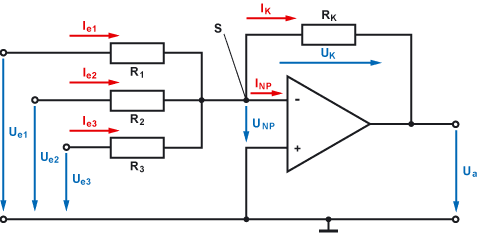
\includegraphics[width=10cm]{pics/Addierer}
%\caption{Beispiel Addiererschaltung \cite{Addierer}}
%\label{Addierer}
%\end{figure}

Nach den Vorgaben der Aufgabenstellung und den goldenen Regeln für den Operationsverstärker \cite{skript} gilt für den invertierenden Addierer:
\begin{equation}
U_{a}=-\,{\frac {10k\Omega }{10\,k\Omega +R_{8}}}\cdot\,U_{H}-\,{\frac {10k
\Omega}{10\,k\Omega +R_{10}}}\cdot\,U_{T}
\end{equation}
Dies bedeutet (bezogen auf Abbildung \ref{spicegesamt}):
\begin{equation}
R_{11}=R_{7}=R_{9}=10\si{k\Omega}
\end{equation}
Das Bauteilwerte der Wiederstände $R_{8} und  R_{10}$ werden später noch verändert.
Dementsprechend wurde nun erstmals die gesamte Schaltung in Spice aufgebaut.\newline

\begin{figure}[h]
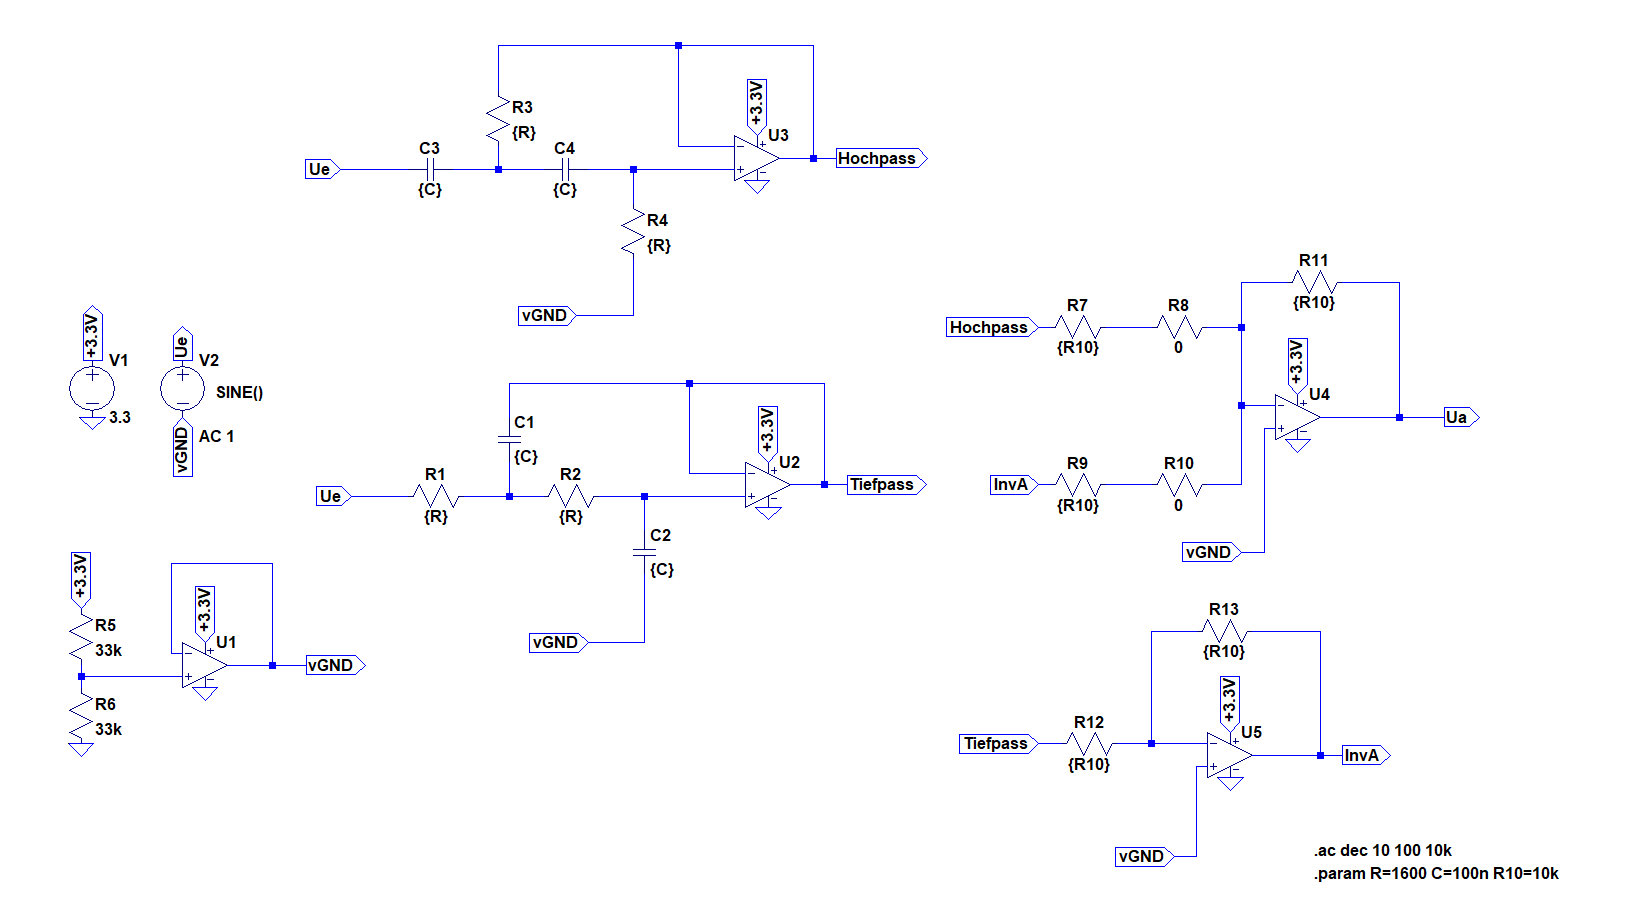
\includegraphics[width=14cm]{pics/SpiceSchaltungGesamt.png}
\caption{Der gesamte Schaltungsaufbau in LT Spice}
\label{spicegesamt}
\end{figure}

\newpage
Außerdem war es ebenfalls Teil der Aufgabe die Schaltung auf dem Breadbord nachzubauen und mit der LENLab Software auszumessen. Diese Bilder zeigen den Aufbau des \textbf{invertierenden Verstärker \ref{invV}} und des \textbf{invertierenden Addierers \ref{invA}.}

\begin{figure}[h]
\centering
\begin{subfigure}{.5\textwidth}
  \centering
  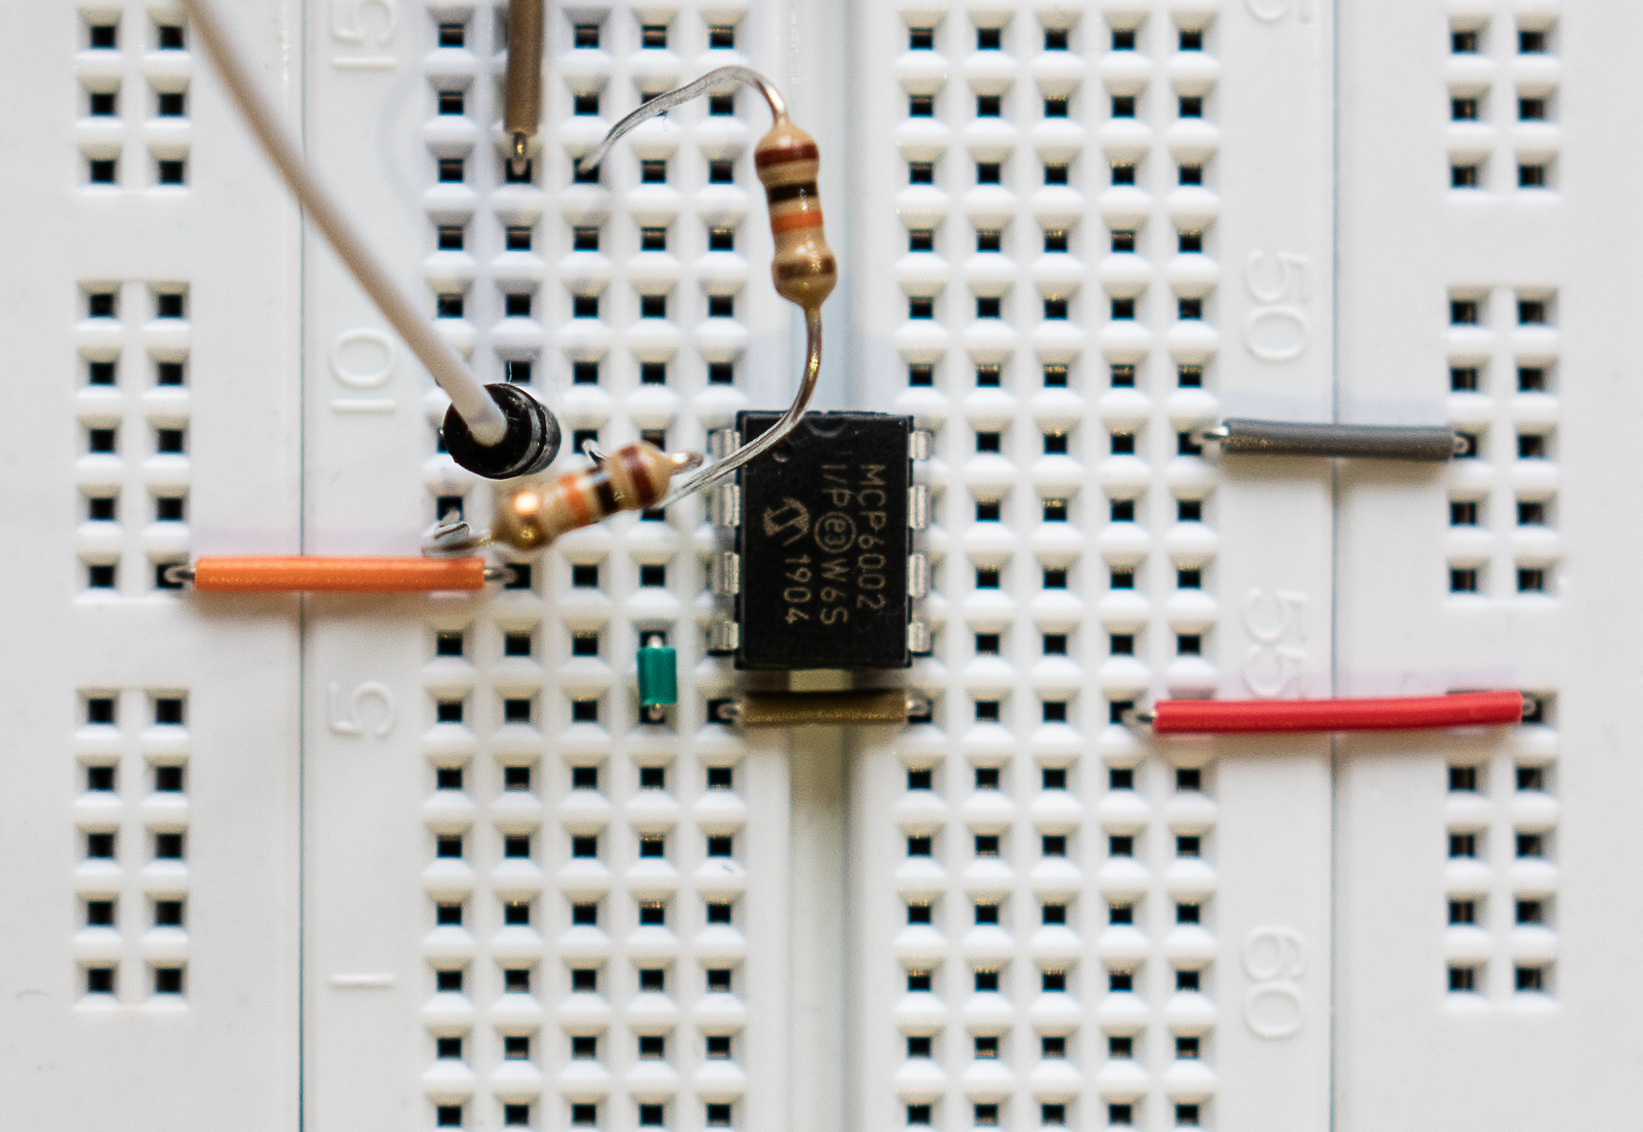
\includegraphics[width=6cm]{pics/Invertierer_aufgebaut.jpg}
  \captionof{figure}{}
  \label{invV}
\end{subfigure}%
\begin{subfigure}{.5\textwidth}
  \centering
  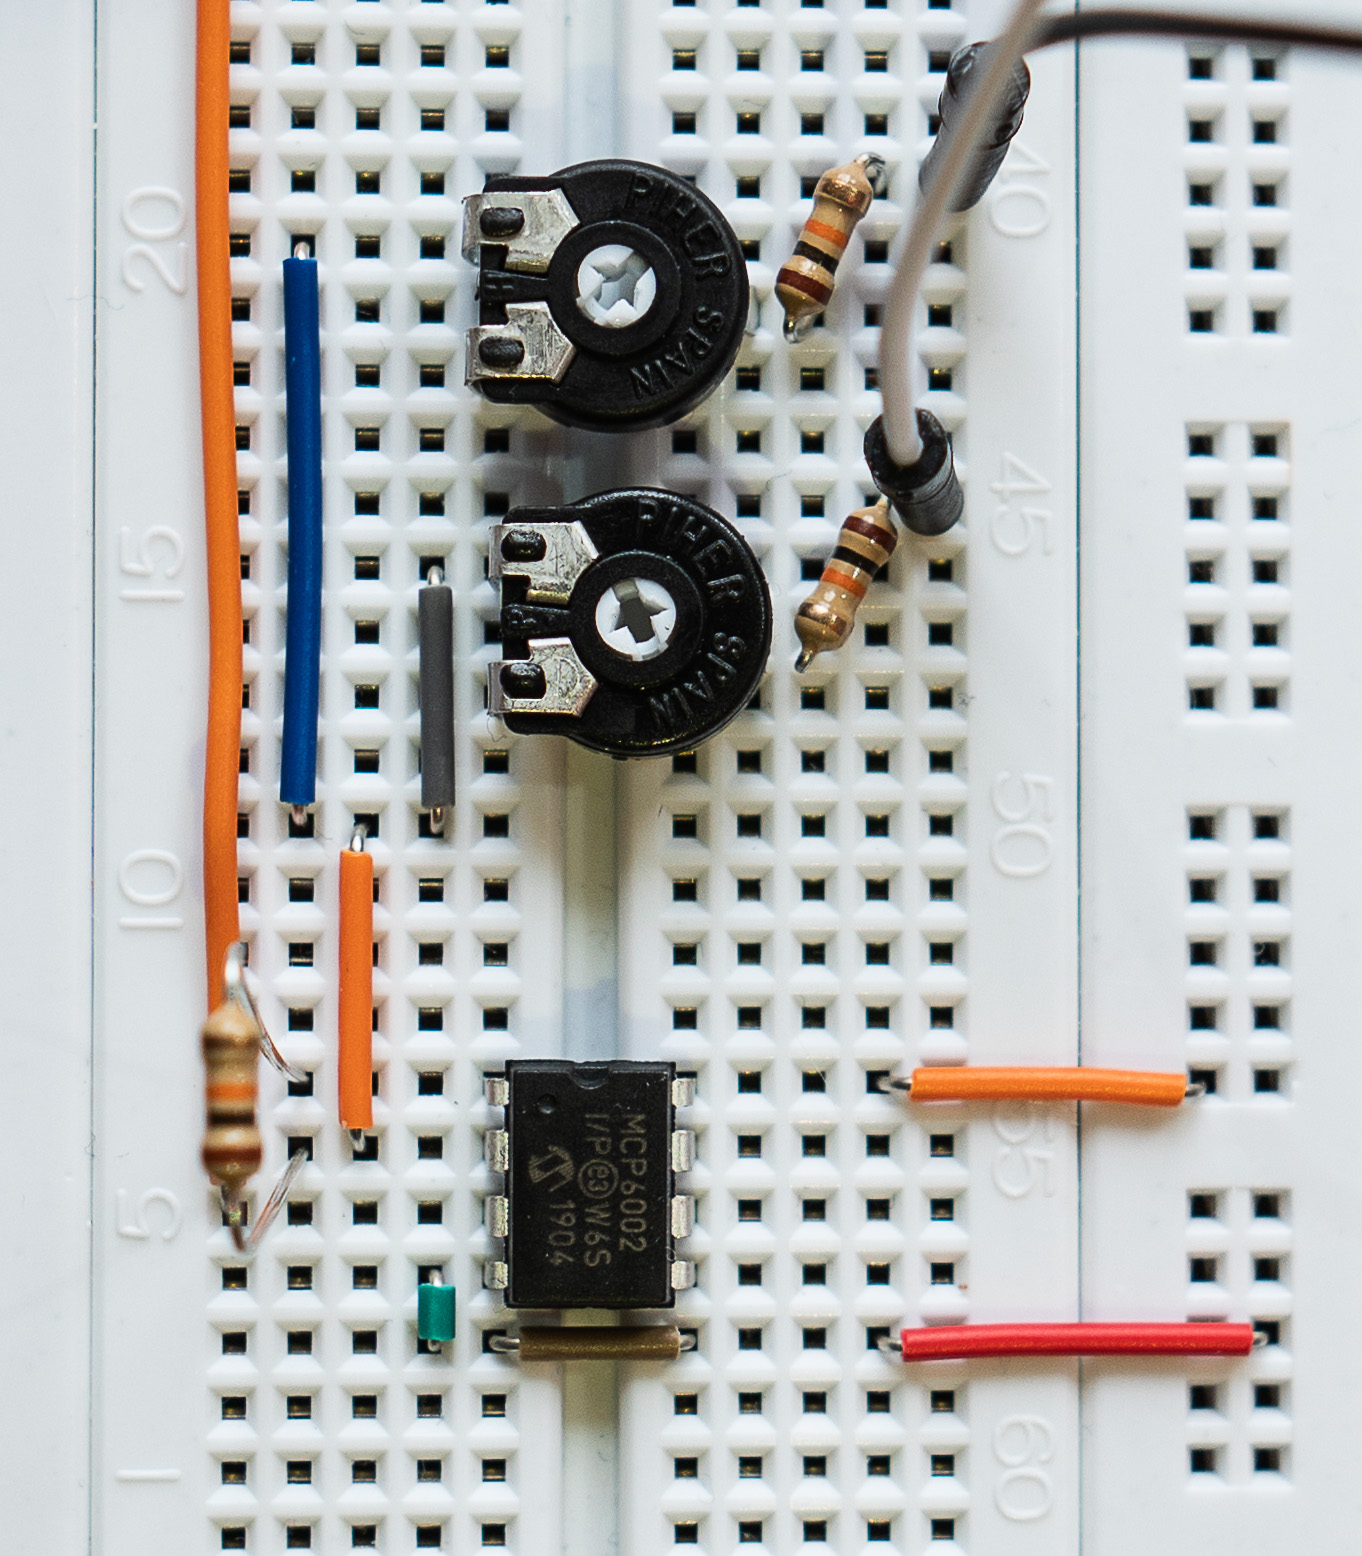
\includegraphics[width=4cm]{pics/Addierer_aufgebaut.jpg}
  \captionof{figure}{}
  \label{invA}
\end{subfigure}
\caption{Invertierender Verstärker (a) und Invertierender Addierer (b)}
\end{figure}

Zur Variation der Widerstände $R_{8}$ und $R_{10}$ wurde für diese Bauteile jeweils ein \newline Potentiometer($\sim 0-100k\Omega$) verbaut, wie es in Abbildung \ref{invA} zu sehen ist.
\newline Sowohl mit dem Schaltungsaufbau in Spice als auch mit der auf dem Breadboard werden Messungen durchgeführt. Deren Ergebnisse im folgenden vorgestellt werden.

\subsection{Ergebnisse}
% A)Simulieren Sie für Werte von R1 = R2 = 0Ω ein Bodediagramm der Gesamtschaltung zwischen 100Hz und 10kHz.
\subsubsection{Aufgabe A}
Simulation eines Bodediagramms der Gesamtschaltung zwischen $\si{100}{Hz}$ und $\si{10}{kHz}$.
\newline $R_{8}$ und $R_{10}$ betragen hierbei $\si{0}{\Omega}$.
\begin{figure}[h]
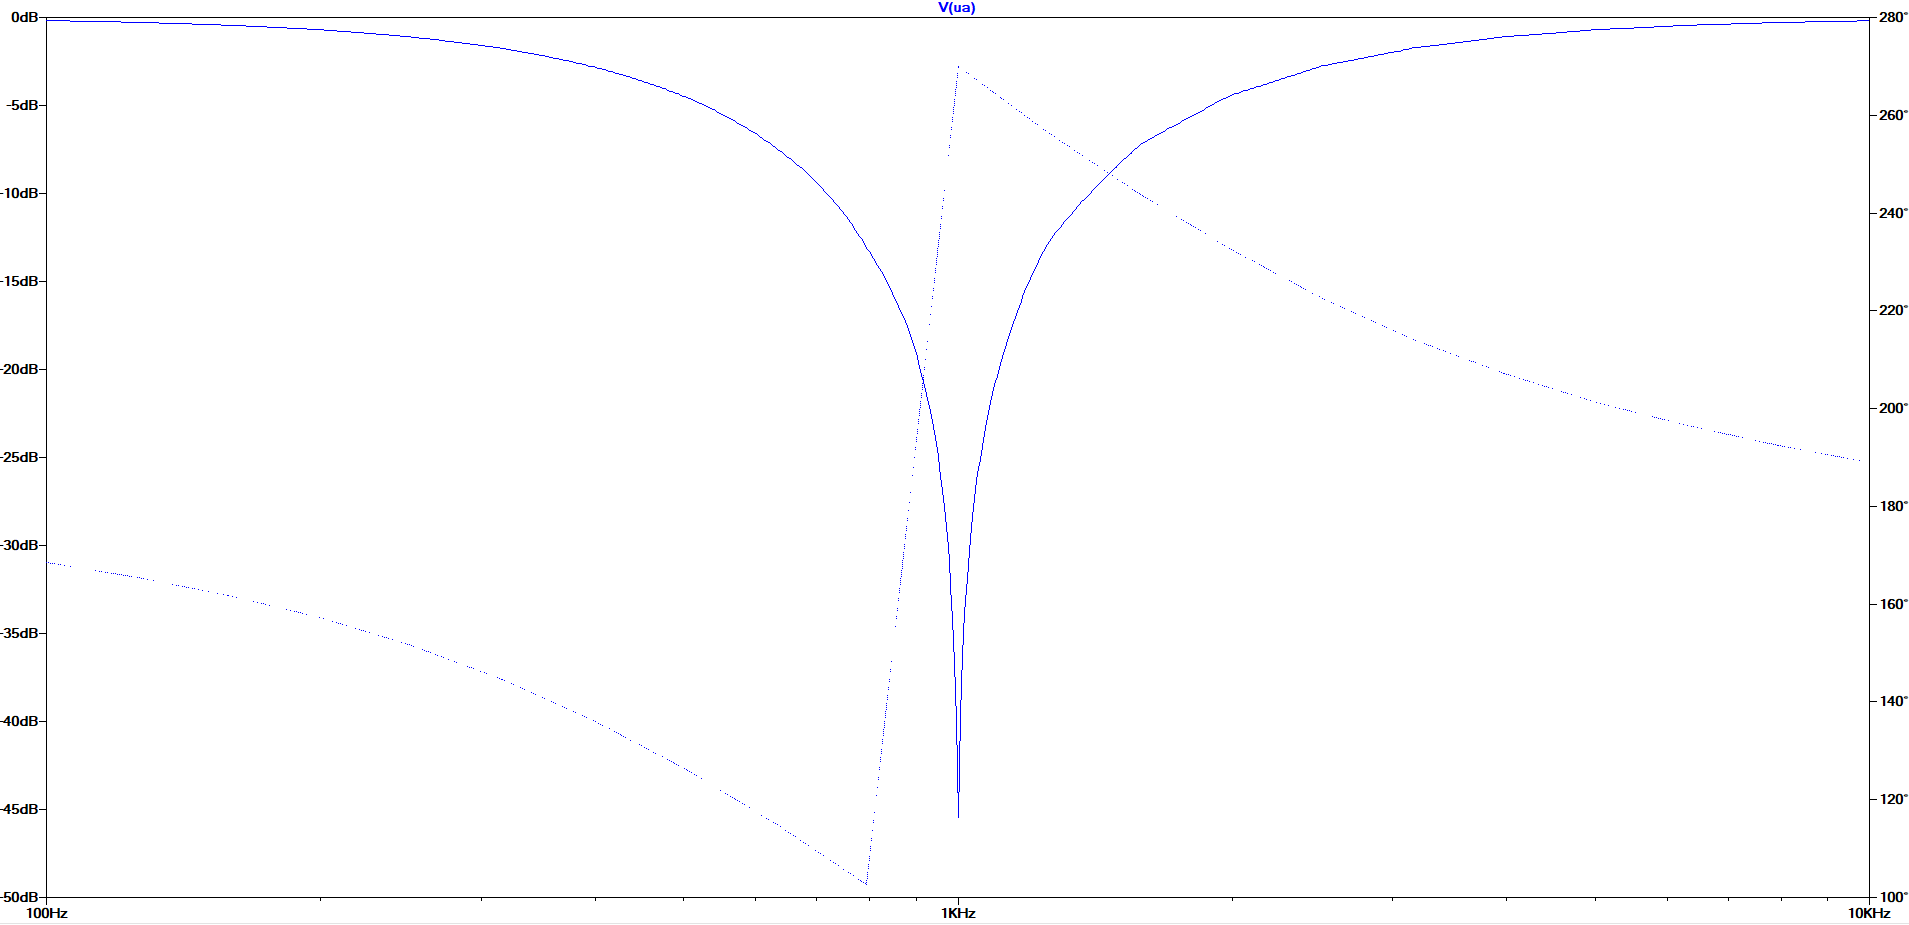
\includegraphics[width=14cm]{pics/BodeAd_ohneInv}
\caption{Das Bodediagramm der Gesamtschaltung ohne invertierenden Verstärker}
\label{bodeA}
\end{figure}

% B) Wie erklären Sie sich den Einbruch des Amplitudengangs bei der Grenzfrequenz Ihrer Filterschaltungen?

% C) Fügen Sie zwischen Tiefpass und Addierschaltung einen invertierenden Verstärker mit Verstärkungsfaktor 1 ein und wiederholen Sie die Simulation aus a). Was beobachten Sie nun? Wie nennt sich ein Filter, welches das beobachtete Übertragungsverhalten aufweist?
\subsubsection{Aufgabe C}
Es wird ein invertierender Verstärkerr zwischen den Ausgang des Tiefpasses und der Addiererschaltung eingebaut. Die Simulation des Bodediagramms der Gesamtschaltung wird wiederholt. $R_{8}$ und $R_{10}$ betragen immernoch $\si{0}{\Omega}$.
\begin{figure}[h]
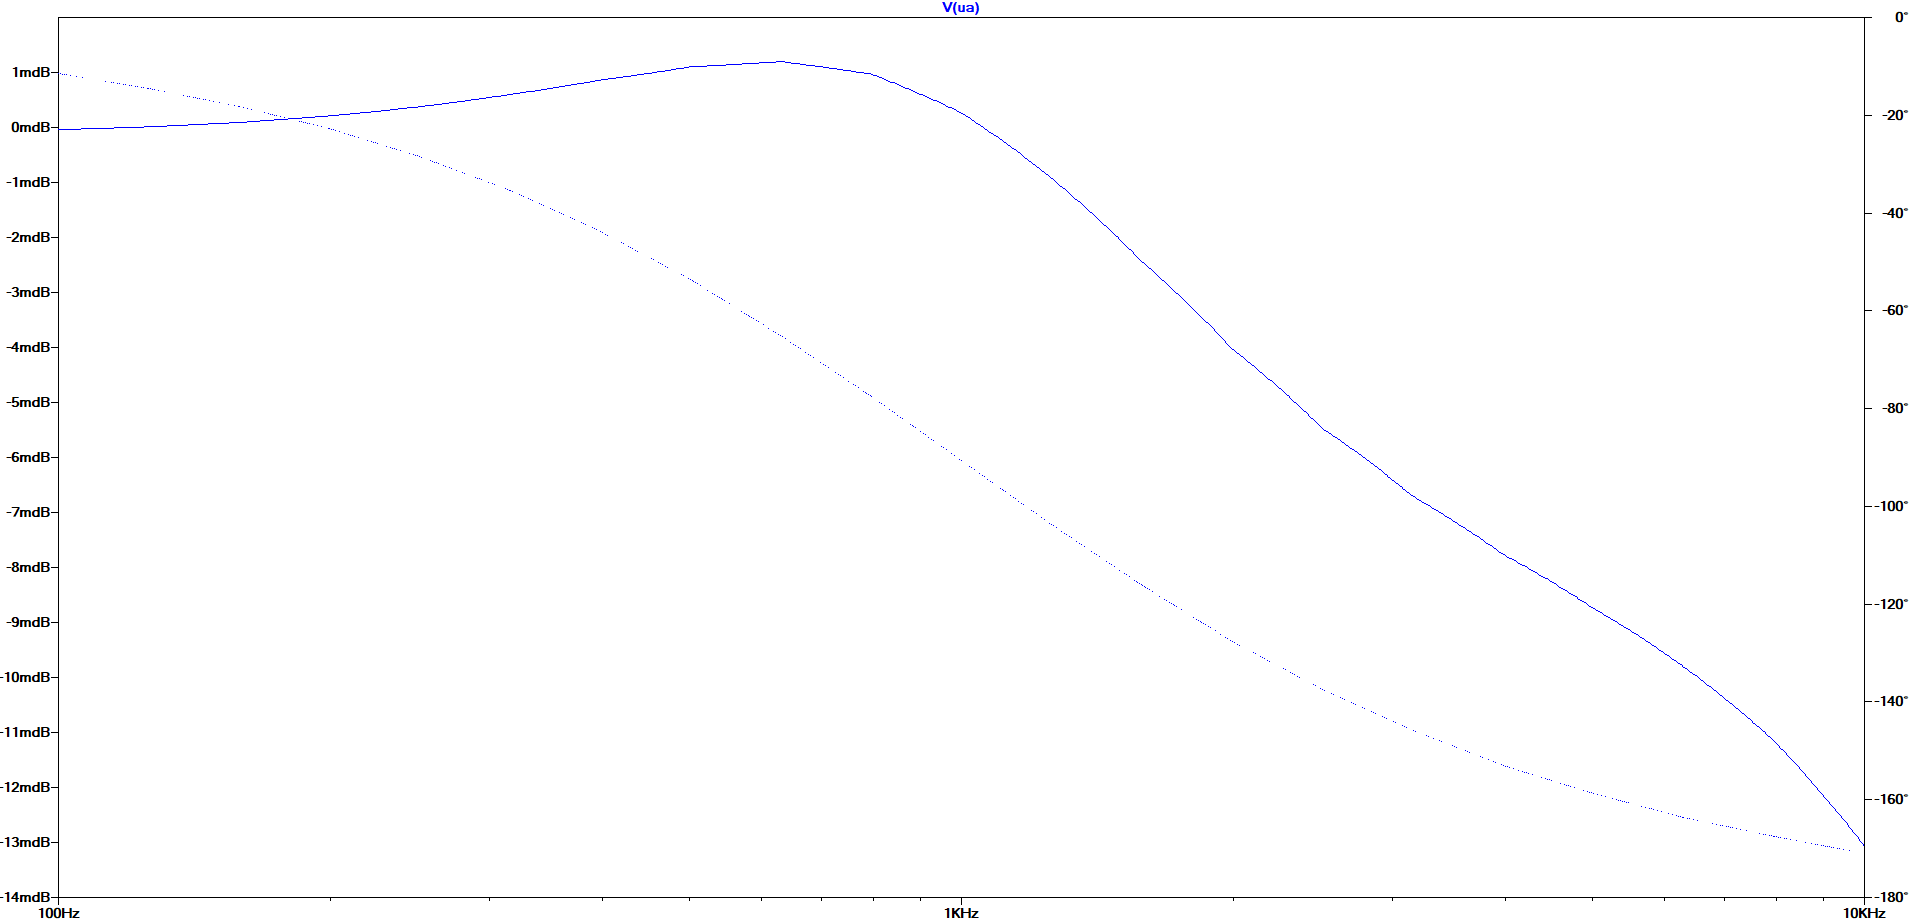
\includegraphics[width=14cm]{pics/BodeAd_mitInv}
\caption{Das Bodediagramm der Gesamtschaltung mit invertierenden Verstärker}
\label{bodeC}
\end{figure}

% D) Simulieren Sie weitere Bodediagramme der Gesamtschaltung für (R1 = 10kΩ, R2 = 90kΩ) und (R1 = 90kΩ, R2 = 10kΩ)
\subsubsection{Aufgabe D}
Es werden weitere Bodediagramme simuliert. Nun werden die Werte für $R_{8}$ und $R_{10}$ entsprechend der Bildbeschriftung variiert.
\begin{figure}[h]
\centering
\begin{subfigure}{.5\textwidth}
  \centering
  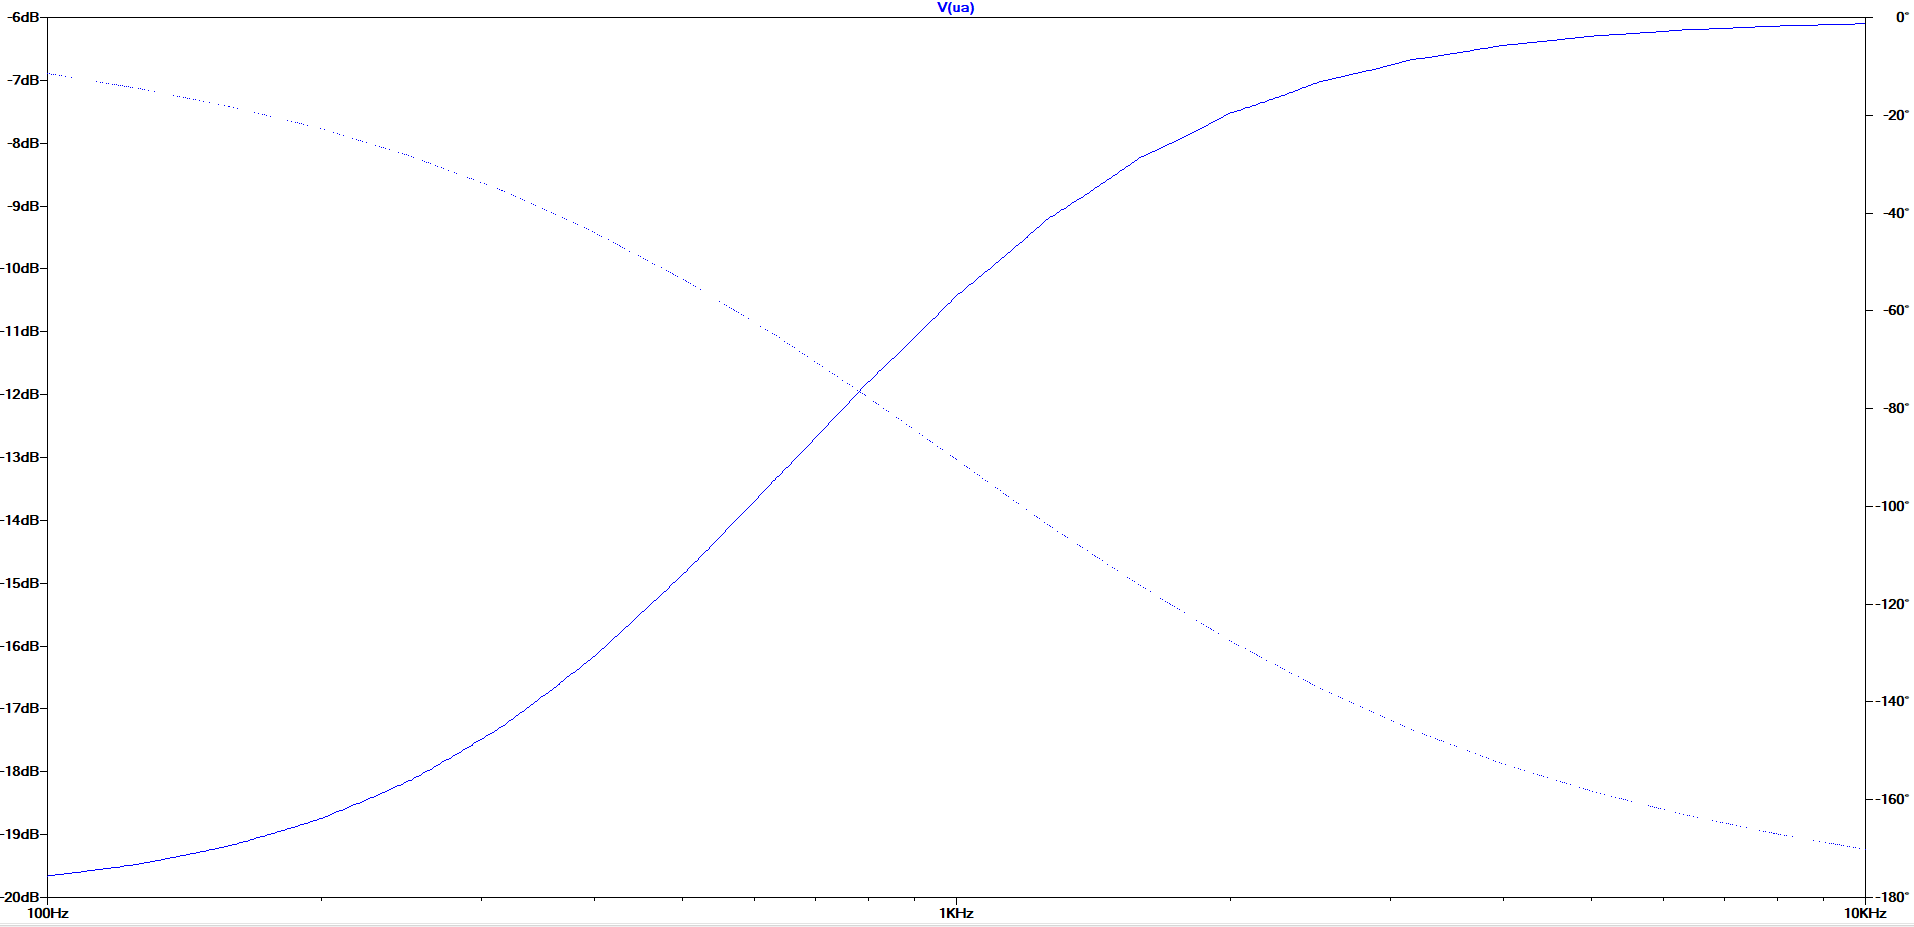
\includegraphics[width=8cm]{pics/10_90}
  \captionof{figure}{Bodediagramm für $R_{8}=\si{10}{\Omega}$ und $R_{10}=\si{90}{\Omega}$}
  \label{Bode1090}
\end{subfigure}%
\begin{subfigure}{.5\textwidth}
  \centering
  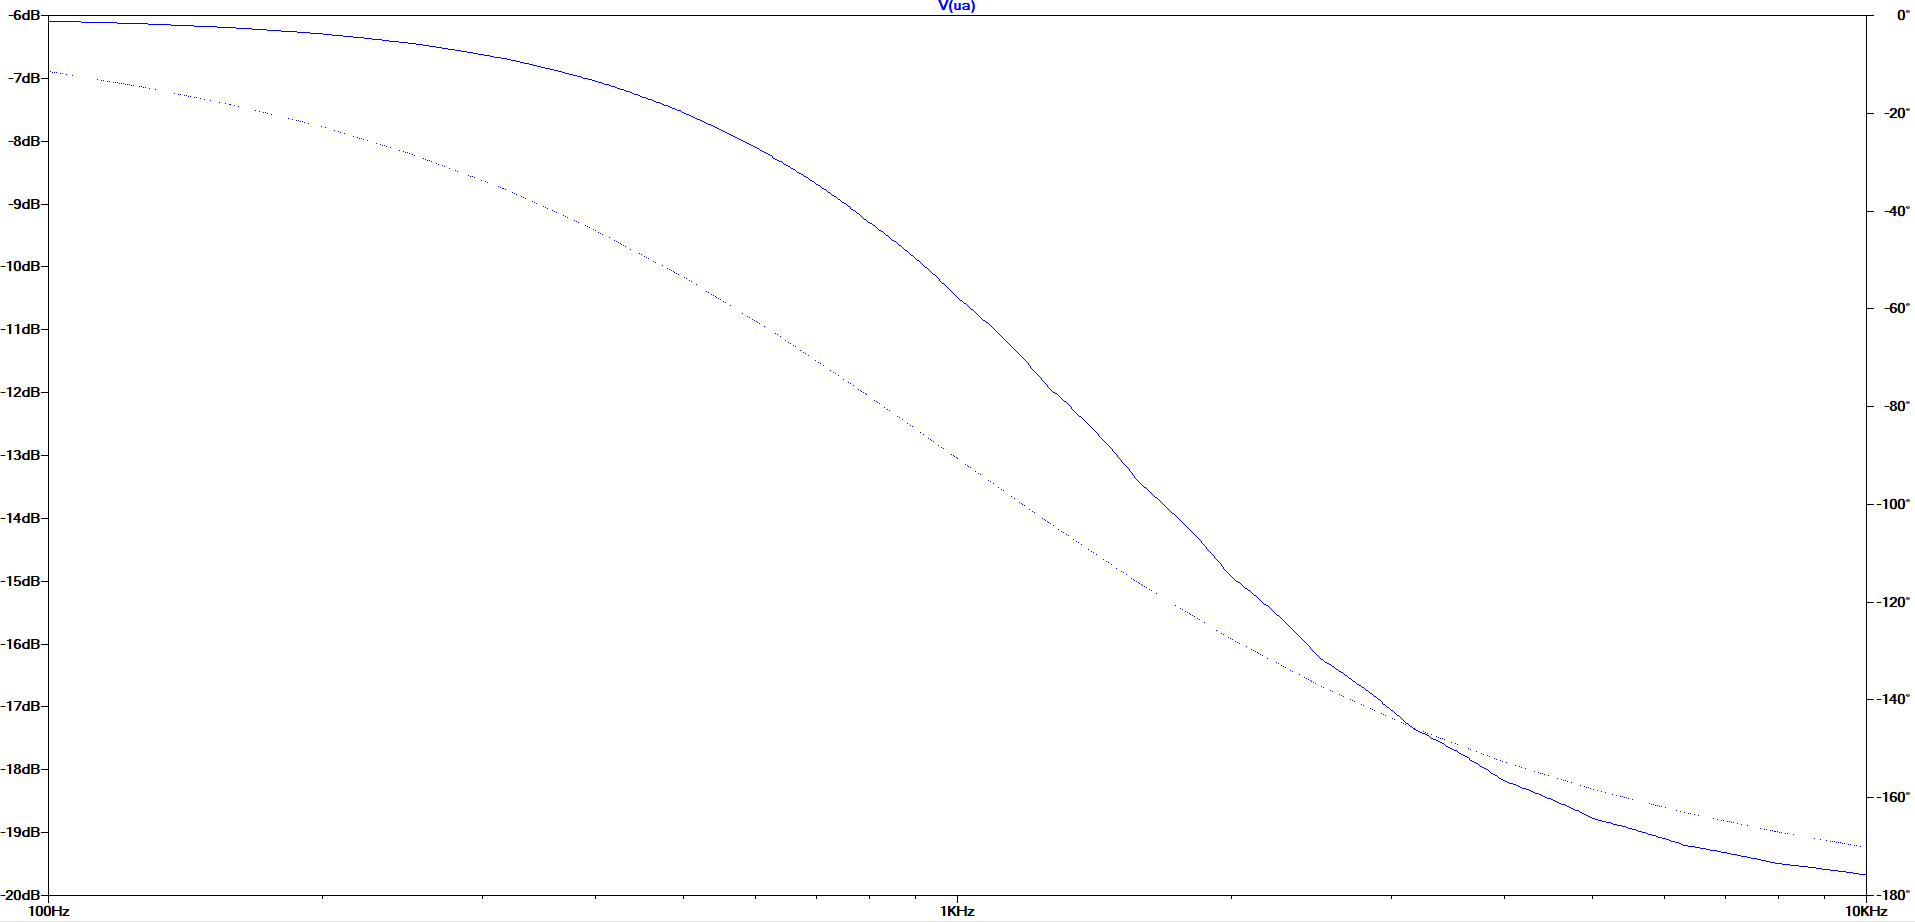
\includegraphics[width=8cm]{pics/90_10}
  \captionof{figure}{Bodediagramm für $R_{8}=\si{90}{\Omega}$ und $R_{10}=\si{10}{\Omega}$}
  \label{Bode9010}
\end{subfigure}
\caption{Bodediagramme für Gesamtschaltung mit variierten Bauteilwerten}
\end{figure}

% E)Bauen Sie die Addierschaltung inklusive invertierendem Verstärker jetzt auch auf Ihrem Steckbrett auf. Verwenden Sie für die Widerstände R1 und R2 die beiden Potentiometer (0...100kΩ)desBauteilsortiments.FührenSieBodediagramm-Messungen derGesamtschaltung für R1 = R2 = 0Ω und bei ein paar weiteren Poti-Einstellungen durch.
\newpage
\subsubsection{Aufgabe E}
Die gesamte Schaltung wurde nun auf dem Steckbrett aufgebaut. Hierbei wurde für $R_{8}$ und $R_{10}$ jeweils ein Potetiometer verbaut. Somit lassen sich die beiden Widerstände stufenlos zwischen $\si{0}{\Omega}$ und $\si{100}{k\Omega}$ verändern. Es folgen sechs Bodediagramm-Messungen mit den angegebenen Bauteilwerten. In \textcolor{blue}{blau ist die Amplitude} und in \textcolor{red}{rot die Phase} aufgetragen. Ein exaktes Einstellen der Potentiometer ist nicht möglich, deshalb werden die Widerstände hier nur gerundet dargestellt.

%Graphik 00 und 100 100
\begin{figure}[h]
\centering
\begin{subfigure}{.5\textwidth}
  \centering
  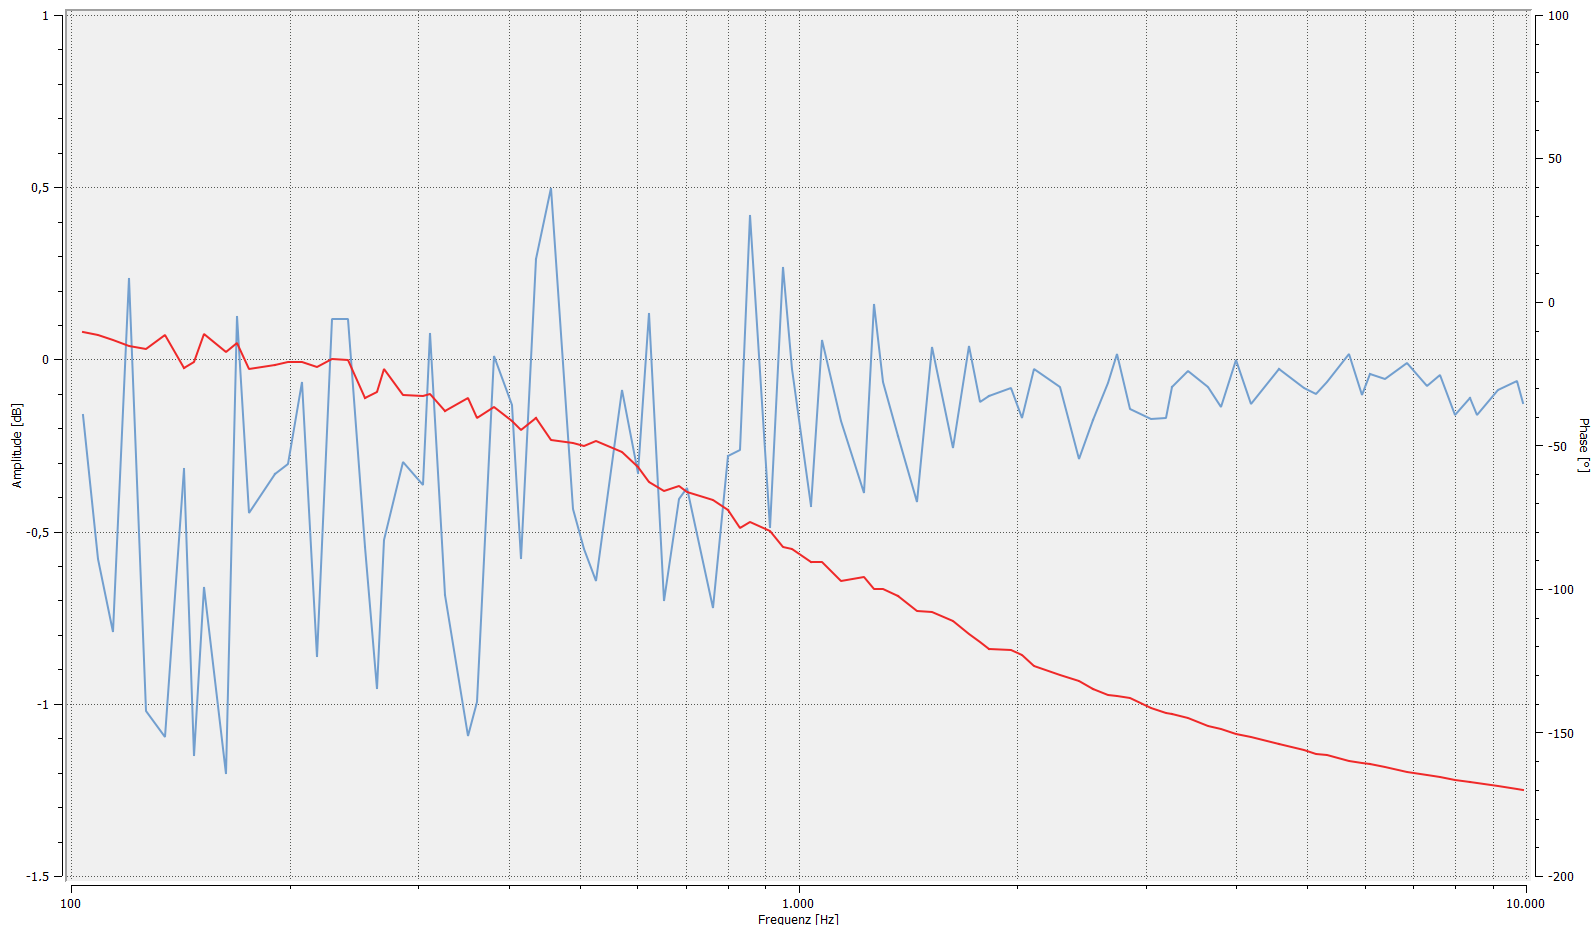
\includegraphics[width=8cm]{pics/0_0Steckbrett}
  \captionof{figure}{Bodediagramm für $R_{8}\approx \si{0}{\Omega}$, $R_{10}\approx \si{0}{\Omega}$}
  \label{0_0SB}
\end{subfigure}%
\begin{subfigure}{.5\textwidth}
  \centering
  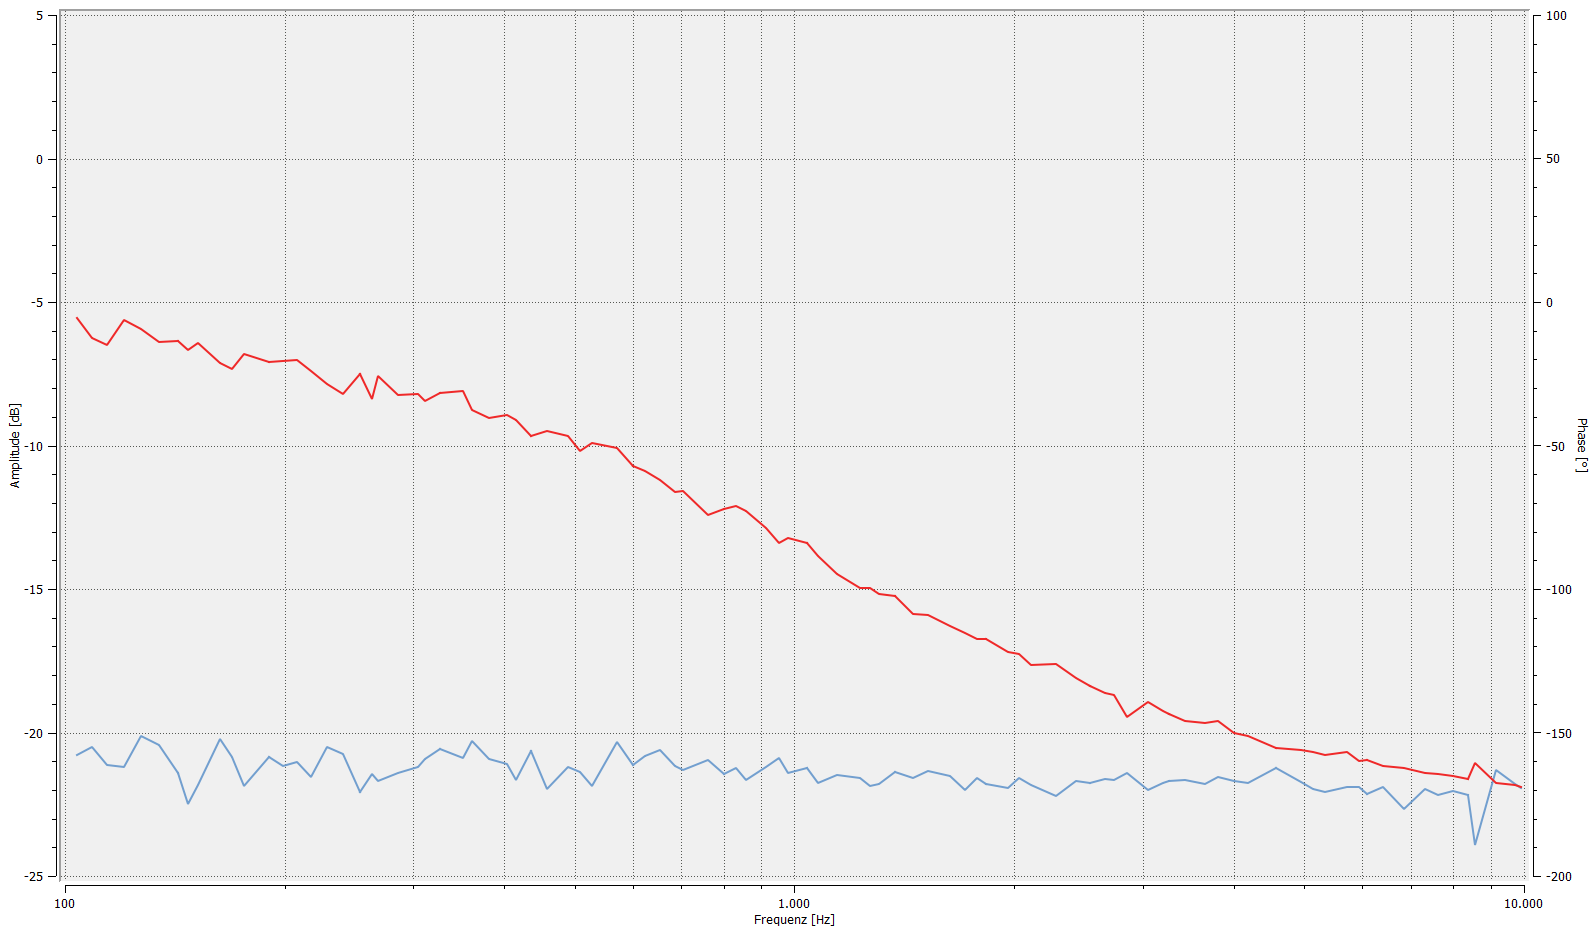
\includegraphics[width=8cm]{pics/100_100Steckbrett}
  \captionof{figure}{Bodediagramm für $R_{8}\approx \si{100}{\,k\Omega}$,$R_{10}\approx \si{100}{\,k\Omega}$}
  \label{1_1SB}
\end{subfigure}
\begin{subfigure}{.5\textwidth}
  \centering
  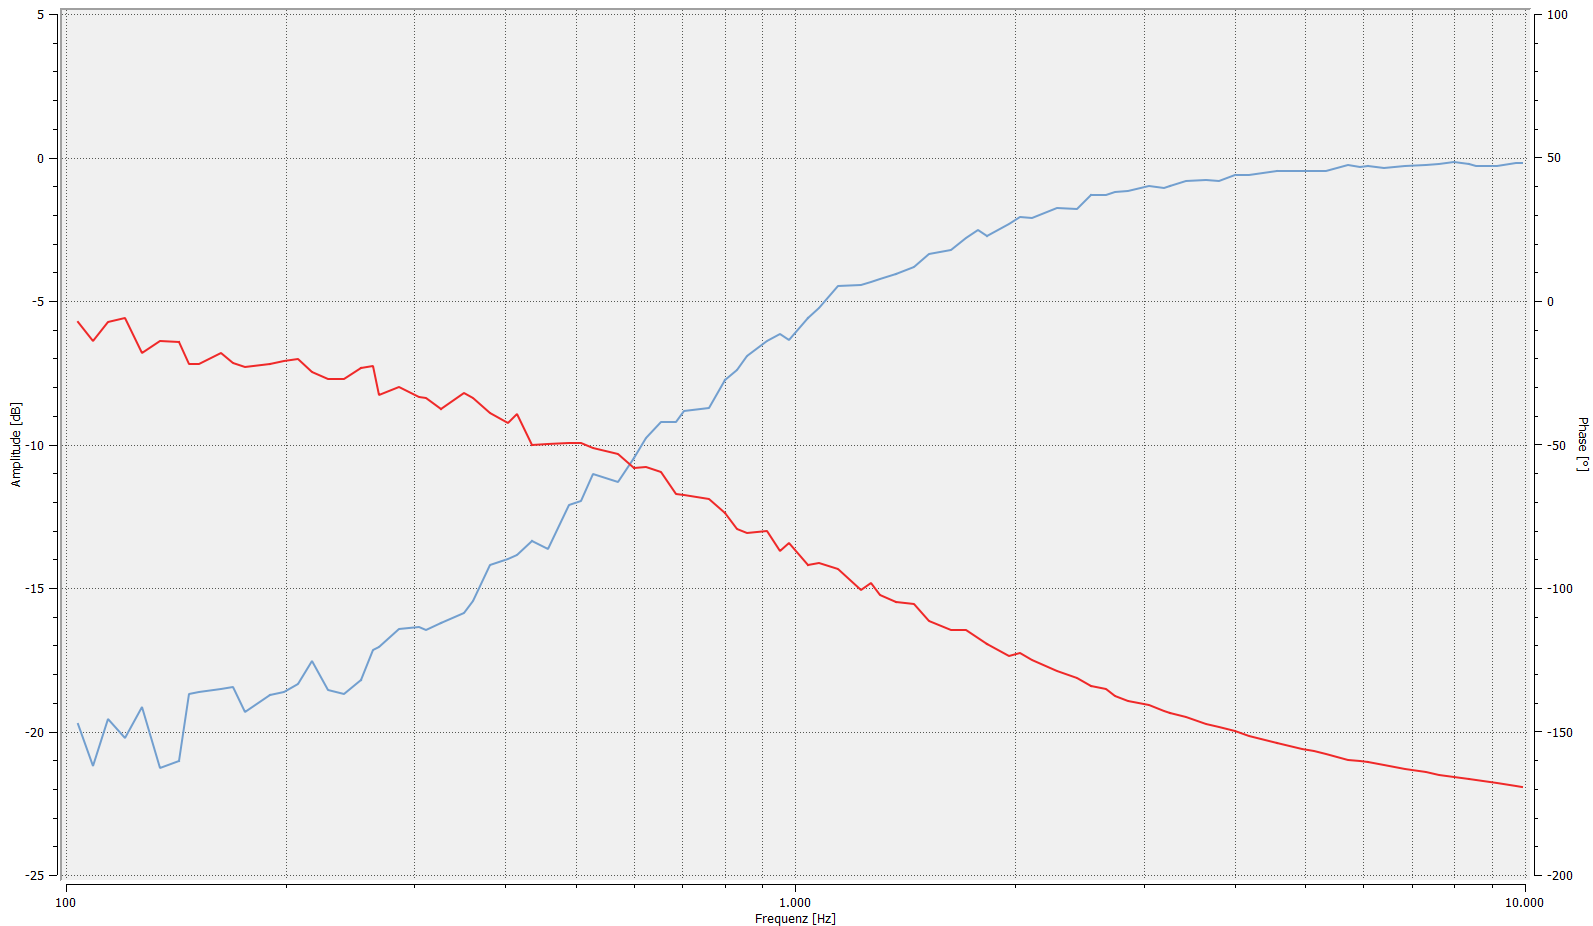
\includegraphics[width=8cm]{pics/0_100Steckbrett}
  \captionof{figure}{Bodediagramm für $R_{8}\approx \si{0}{\Omega}$, $R_{10}\approx \si{100}{\,k\Omega}$}
  \label{0_1SB}
\end{subfigure}%
\begin{subfigure}{.5\textwidth}
  \centering
  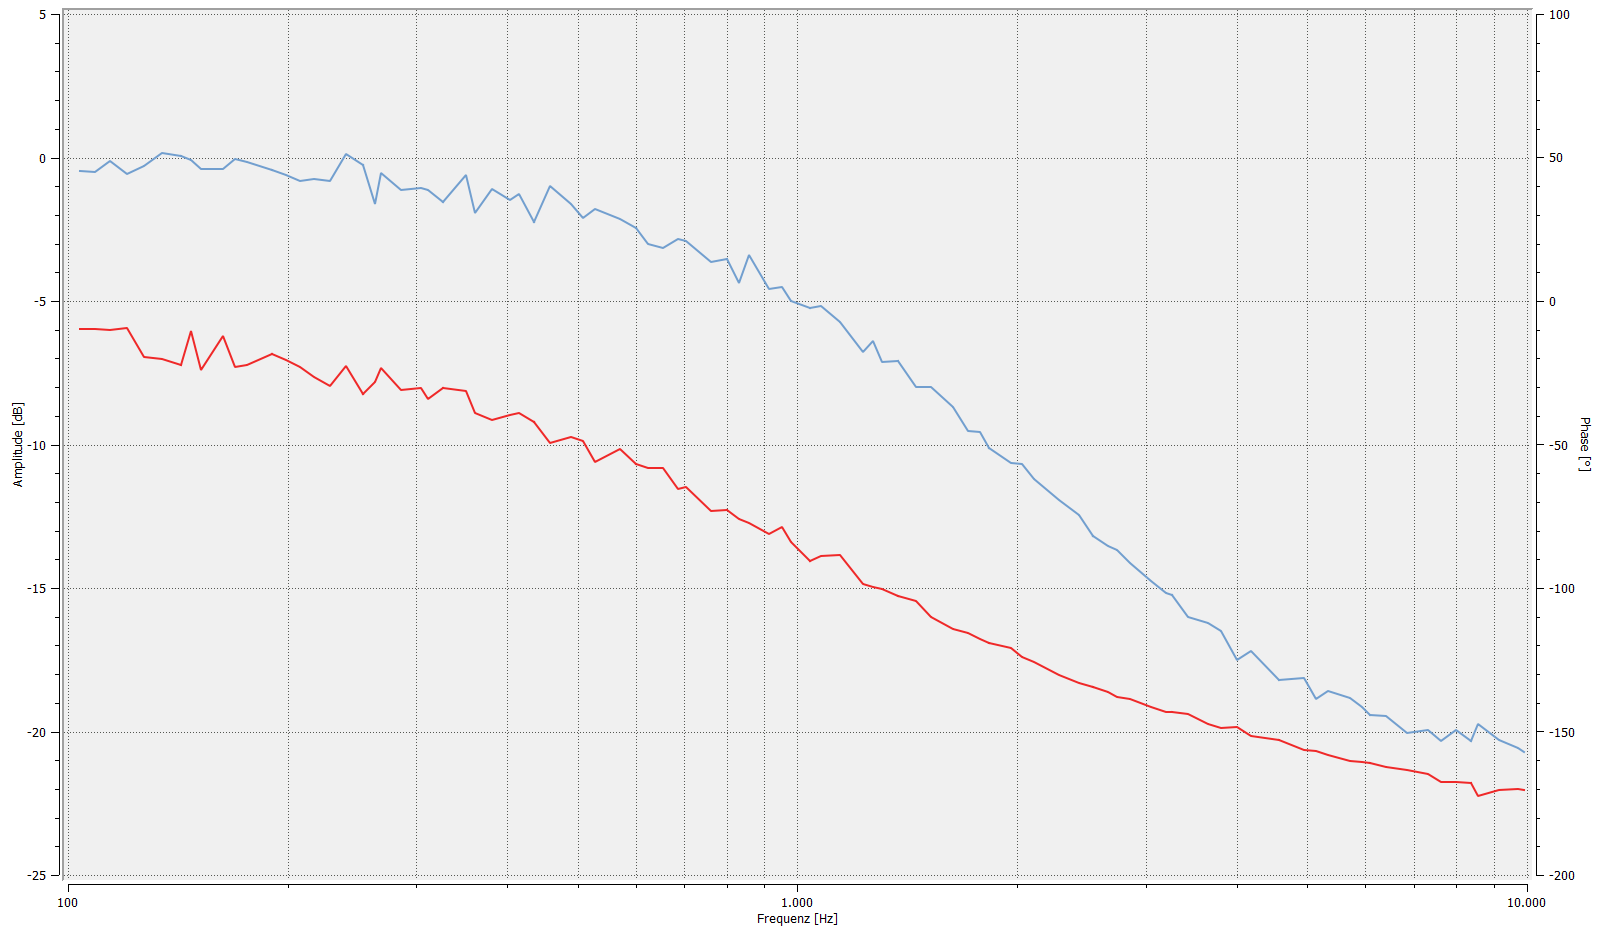
\includegraphics[width=8cm]{pics/100_0Steckbrett}
  \captionof{figure}{Bodediagramm für $R_{8}\approx \si{100}{\,k\Omega}$, $R_{10}\approx \si{0}{\Omega}$}
  \label{1_0SB}
\end{subfigure}
\begin{subfigure}{.5\textwidth}
  \centering
  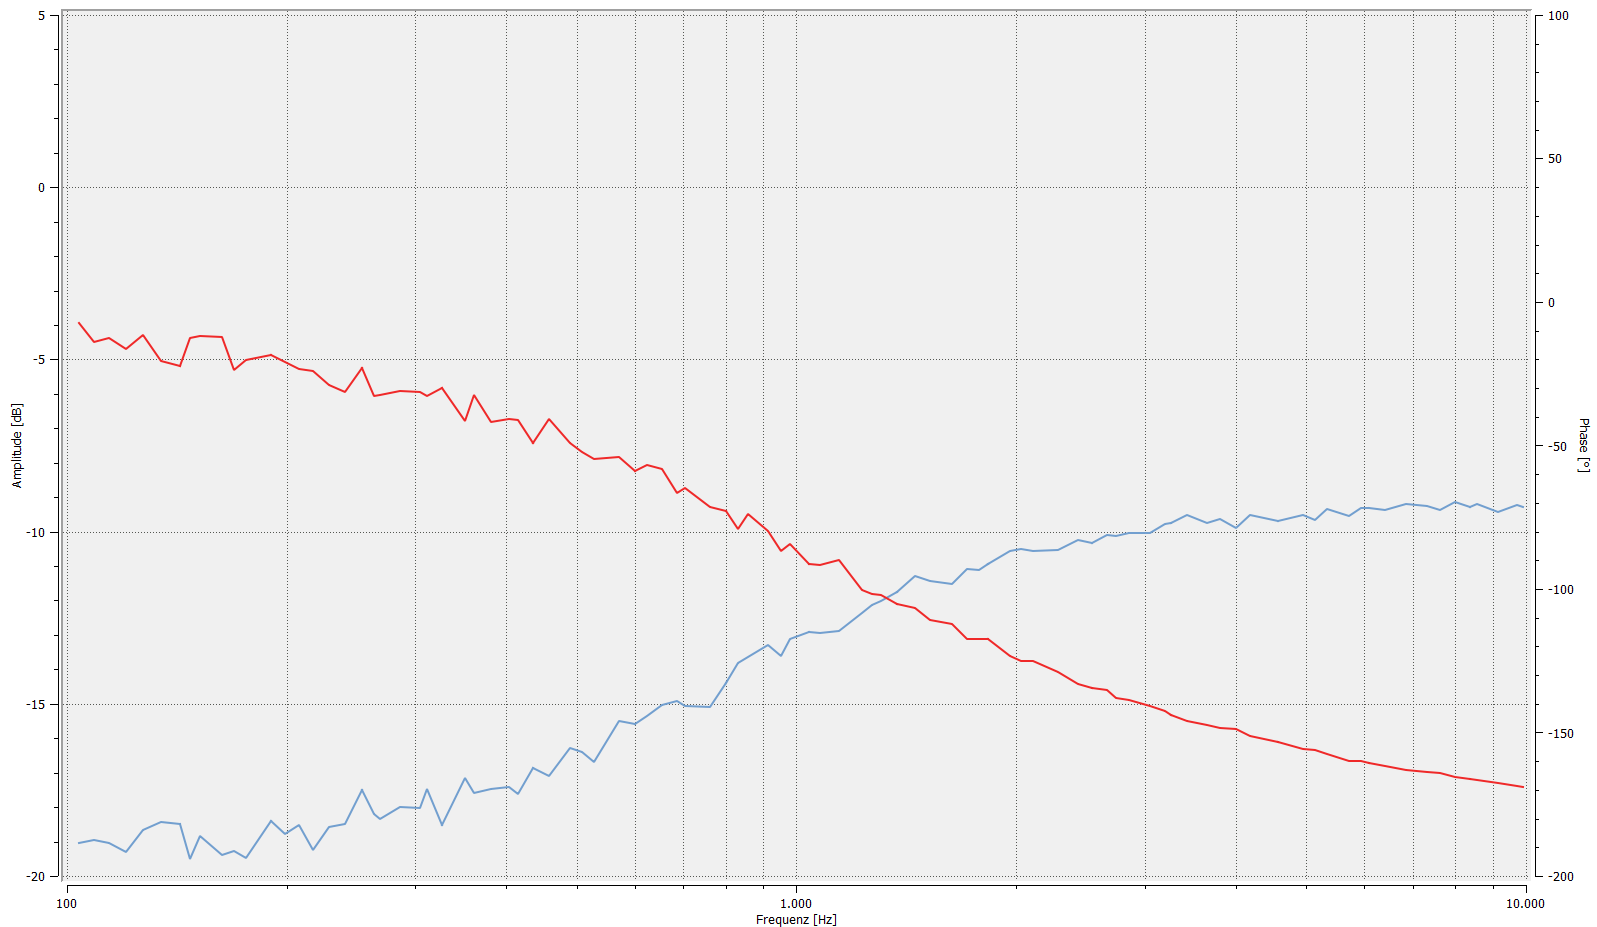
\includegraphics[width=8cm]{pics/30_60Steckbrett}
  \captionof{figure}{Bodediagramm für $R_{8}\approx \si{30}{\,k\Omega}$, $R_{10}\approx \si{60}{\,k\Omega}$}
  \label{3_6SB}
\end{subfigure}%
\begin{subfigure}{.5\textwidth}
  \centering
  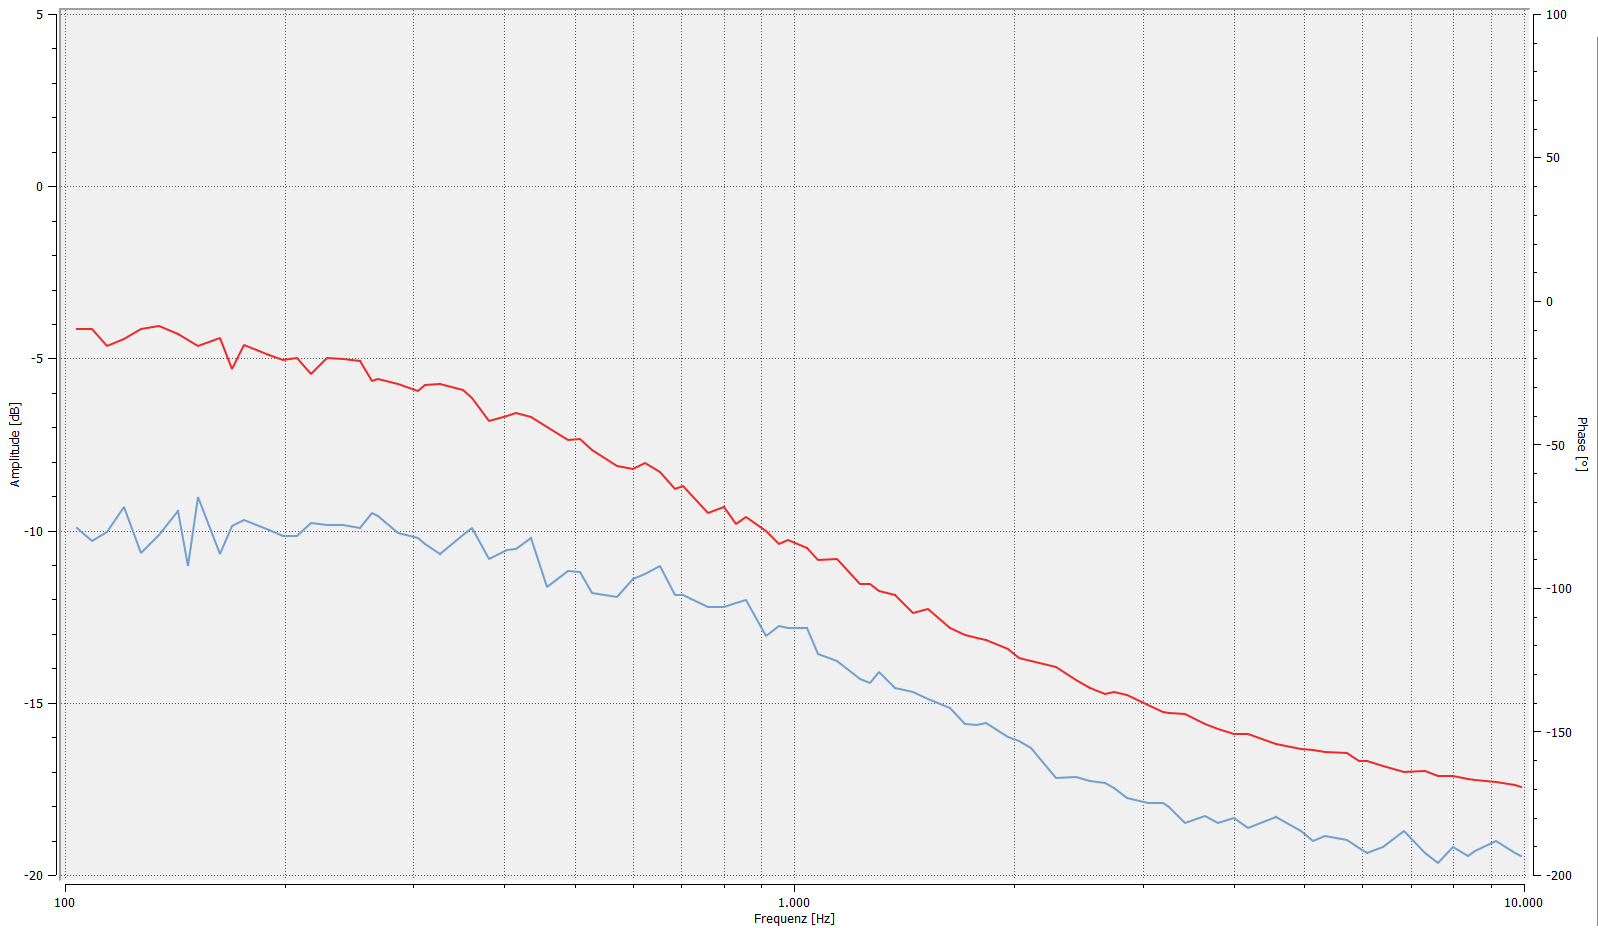
\includegraphics[width=8cm]{pics/60_30Steckbrett}
  \captionof{figure}{Bodediagramm für $R_{8}\approx \si{60}{\,k\Omega}$, $R_{10}\approx \si{30}{\,k\Omega}$}
  \label{6_3SB}
\end{subfigure}

\caption{Bodediagramme für Gesamtschaltung mit Potentiometer von $R_{8}$ und $R_{10}$}
\end{figure}
\newpage
% F)  Nun sollen zwei Sinussignale verschiedener Frequenz überlagert und auf den Eingang des Equalizers gegeben werden. Nutzen Sie zur Überlagerung die gleiche Schaltung wie in Abbildung 4, jedoch mit Kanal A und Kanal B des DAC an den beiden Enden des Spannungsteilers.ErzeugenSiemitdemSignalgeneratoranKanalAeineFrequenzvon ca. 250Hz. An Kanal B soll ein Sinus mit ca. 5kHz ausgegeben werden. Dies erreichen Sie, indem Sie einen Frequenzmultiplikator für Kanal B von 20 einstellen. Nehmen Sie mit dem Oszilloskop das Eingangssignal und die Ausgangssignale bei den beiden Extremstellungen auf (R1 = 0Ω, R2 = 100kΩ und umgekehrt).

\subsubsection{Aufgabe F}
Zwei sich überlagernde Sinussignale mit den Frequenzen $\si{250}{Hz}$ und $\si{5}{\,k\Omega}$ werden in die Steckbrettschaltung hinein geschickt. Nun wird das Eingangs- und Ausgangssignal jeweils für die Einstellungen $R_{8}=\si{0}{\Omega}$, $R_{10}=\si{100}{\,k\Omega}$ und $R_{8}=\si{100}{\,k\Omega}$, $R_{10}=\si{0}{\Omega}$ aufgezeichnet.

\begin{figure}[h]
\centering
\begin{subfigure}{1\textwidth}
\centering
  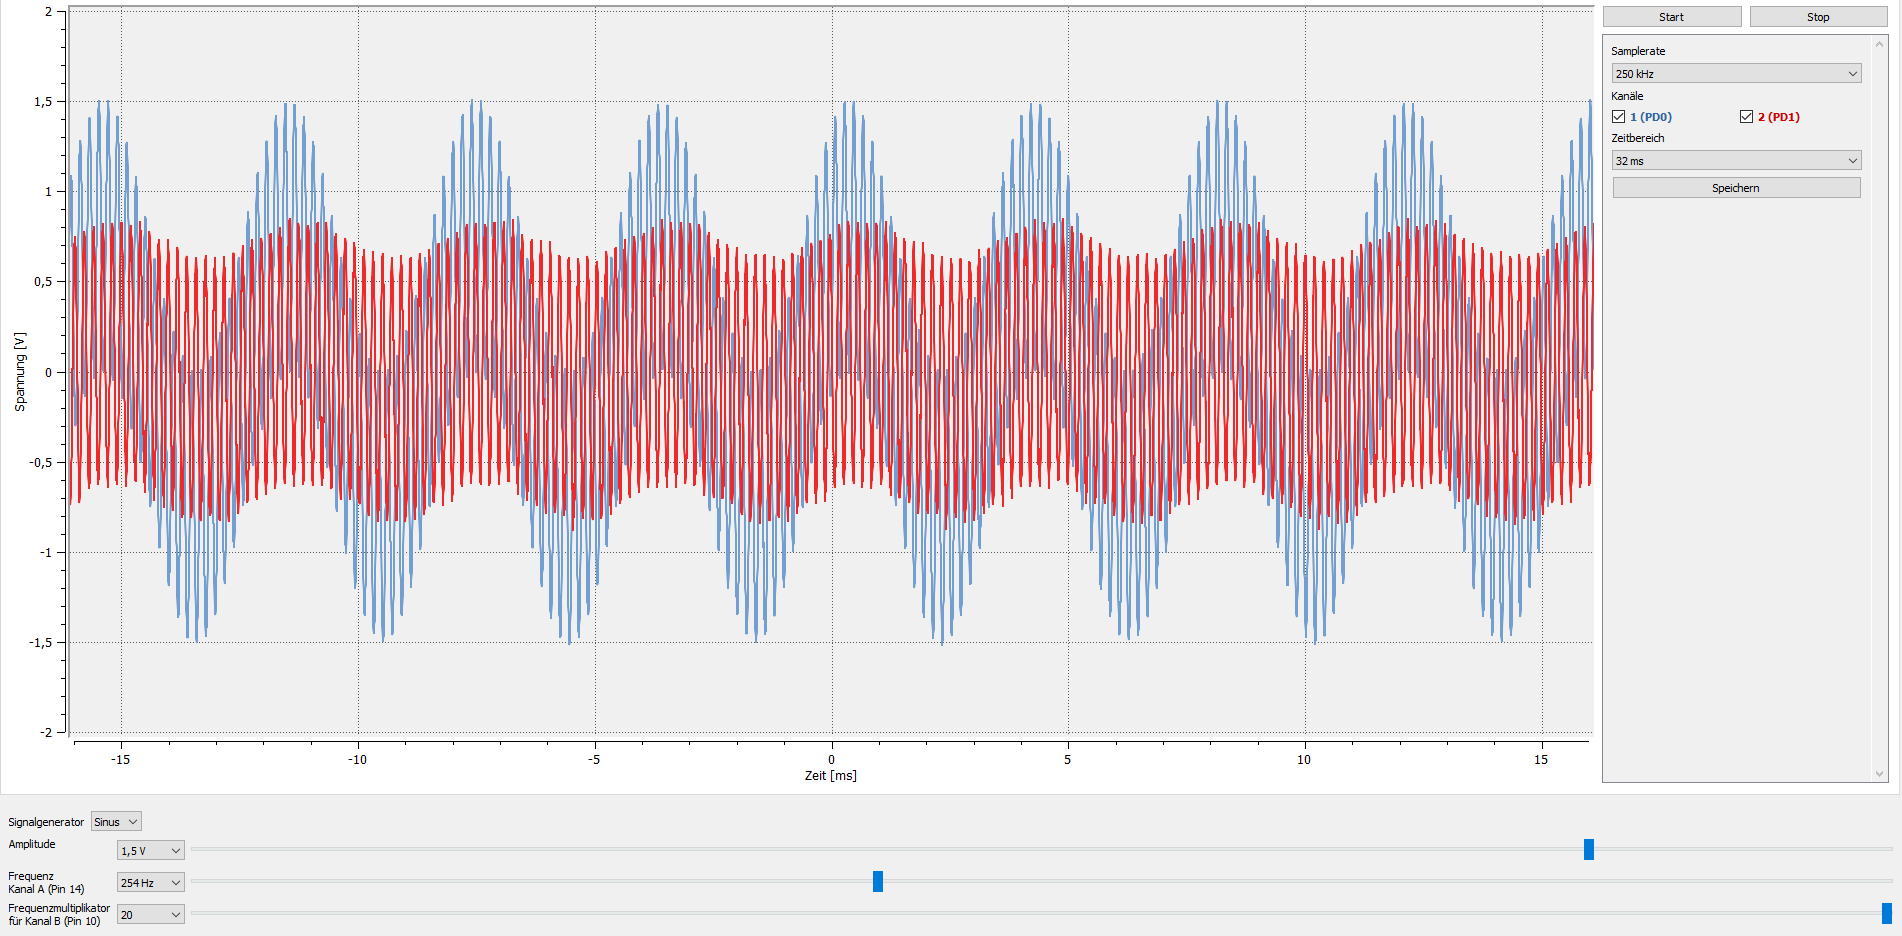
\includegraphics[width=17cm]{pics/3.3f_0_100}
  \captionof{figure}{Oszilloskop für $R_{8}=\si{0}{\Omega}$ und $R_{10}=\si{100}{\,k\Omega}$}
  \label{sin0_1}
\end{subfigure}
\begin{subfigure}{1\textwidth}
\centering
  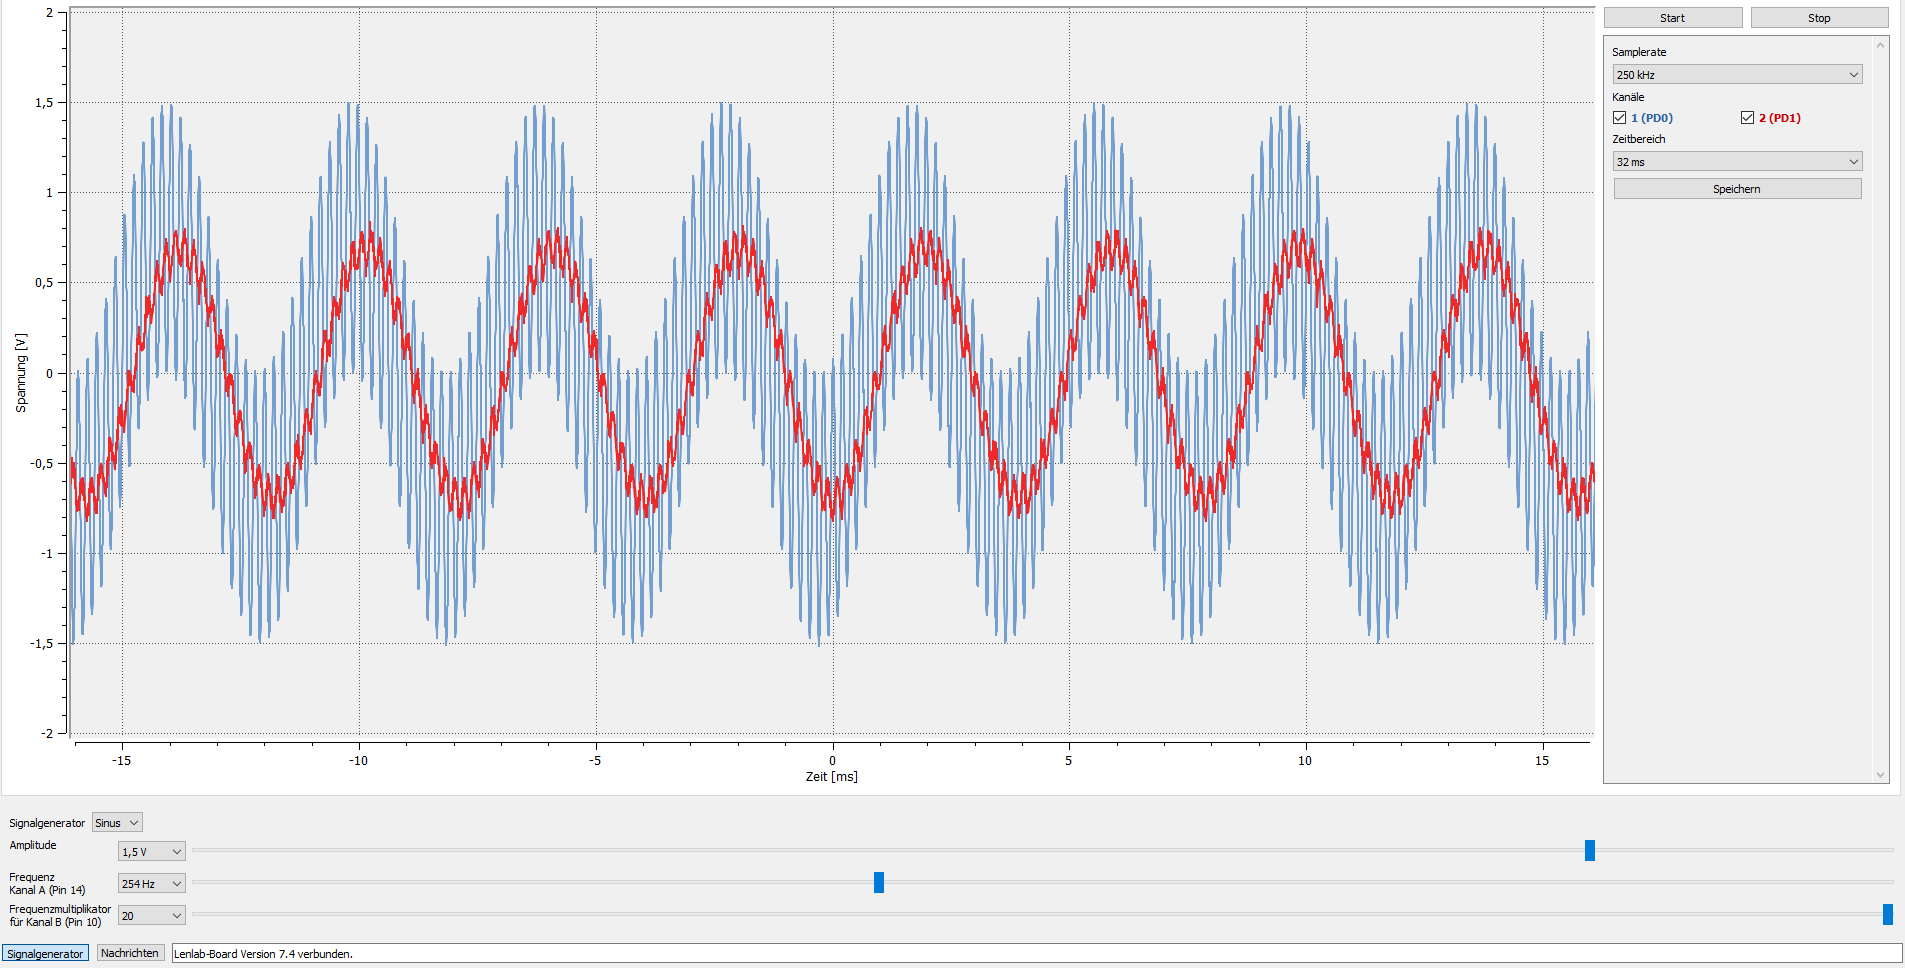
\includegraphics[width=17cm]{pics/3.3f_100_0}
  \captionof{figure}{Oszilloskop für $R_{8}=\si{100}{\,k\Omega}$ und $R_{10}=\si{0}{\Omega}$}
  \label{sin1_0}
\end{subfigure}
\caption{Oszilloskop für Sinussignal}
\end{figure}



\subsection{Diskussion}




